\chapter{Documentación de la interfaz}


La interfaz tiene una finalidad simple y no es el objetivo del trabajo.  Sin embargo, en este apéndice detallamos el código de la interfaz: su estructura y las dependencias necesarias para poder ser utilizada.

\section{Estructura de la interfaz}

A continuación, comentamos la implementación y diseño de la interfaz. Mostraremos su diagrama de clases y comentaremos sus funciones.

\subsection{Diagrama de clases}

La interfaz tiene una estructura de ficheros modular separando un fichero principal \textbf{main} de otros ficheros que se encargan de la inferencia. Los programas que se encargan de utilizar los modelos para inferir son \textbf{model definition} y \textbf{predictions}. 
\begin{itemize}
	\item \textbf{Model definition}. Este fichero reúne el código necesario para definir los modelos.
	\item \textbf{Predictions}. Utiliza la instancia del \textbf{Learner} de \textbf{Model definition} para hacer la predicción final.
\end{itemize}

En un diagrama de clases mostraremos todos los ficheros representados como metaclases que contienen a su vez sus propias clases. Dentro de la definición de la metaclase o fichero \textbf{model definition} representaremos como un cuadro instancia todas las clases y métodos necesarios para las arquitectura y modelos que definimos en la Figura 4.1.

A continuación, mostraremos el diagrama de clases de toda la interfaz.

\begin{figure}[H]
	\centering
	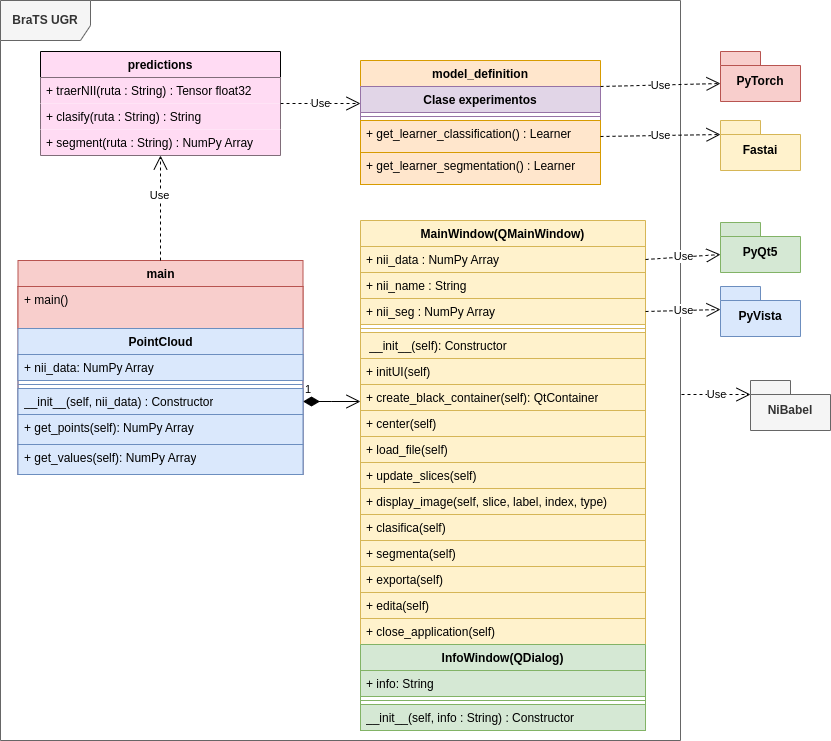
\includegraphics[width=1.0\linewidth]{imagenes/diagrama_interfaz.png}
	\caption{Diagrama de clases de toda la interfaz}
\end{figure}

En la figura B.1, observamos el diagrama de clases de la interfaz. Las relaciones en este diagrama es como podemos ver la metaclase principal que instancia la ventana de la interfaz para interir utiliza a \textbf{predictions} y este a su vez utiliza a \textbf{model definition}. Además se observa como la metaclase de la definición del modelo utiliza a PyTorch y a FastAI. Y como la clase de la ventana principal usa \textbf{PyQt5} y \textbf{PyVista}. Finalmente, se observa como todas las clases usan a la librería \textbf{NiBabel}.


\subsection{Documentación de funciones}

En el siguiente apartado, creamos una lista con las funciones implicadas en cada clase. Comentaremos su función y lo que devuelve.

\begin{itemize}
	\item \textbf{predictions}
	\begin{itemize}
		\item \texttt{traerNII(ruta : String) : Tensor float32} \\
		Esta función recibe una cadena que representa la ruta de un archivo NII y devuelve un tensor de tipo float32.
		
		\item \texttt{clasify(ruta : String) : String} \\
		Esta función toma como parámetro una cadena con la ruta de un archivo y devuelve una cadena con la clasificación resultante.
		
		\item \texttt{segment(ruta : String) : NumPy Array} \\
		Esta función recibe una cadena que representa la ruta de un archivo y devuelve un arreglo de tipo NumPy con la segmentación resultante.
	\end{itemize}
	
	\item \textbf{main}
	\begin{itemize}
		\item \texttt{main()} \\
		Función principal que inicia la ejecución del programa.
	\end{itemize}
	
	\item \textbf{PointCloud}
	\begin{itemize}
		\item \texttt{PointCloud(nii\_data : NumPy Array)} \\
		Constructor de la clase \texttt{PointCloud} que recibe como parámetro un arreglo de tipo NumPy.
		
		\item \texttt{get\_points() : NumPy Array} \\
		Esta función devuelve un arreglo de tipo NumPy con los puntos de la nube de puntos.
		
		\item \texttt{get\_values() : NumPy Array} \\
		Esta función devuelve un arreglo de tipo NumPy con los valores correspondientes a la nube de puntos.
	\end{itemize}
	
	\item \textbf{model\_definition}
	\begin{itemize}
		\item \texttt{get\_learner\_classification() : Learner} \\
		Esta función devuelve un objeto de tipo \texttt{Learner} para la clasificación.
		
		\item \texttt{get\_learner\_segmentation() : Learner} \\
		Esta función devuelve un objeto de tipo \texttt{Learner} para la segmentación.
	\end{itemize}
	
	\item \textbf{MainWindow(QMainWindow)}
	\begin{itemize}
		\item \texttt{MainWindow()} \\
		Constructor de la clase \texttt{MainWindow}.
		
		\item \texttt{initUI()} \\
		Inicializa la interfaz de usuario.
		
		\item \texttt{create\_black\_container(self) : QtContainer} \\
		Crea un contenedor de color negro.
		
		\item \texttt{center()} \\
		Centra la ventana principal.
		
		\item \texttt{load\_file()} \\
		Carga un archivo.
		
		\item \texttt{update\_slices()} \\
		Actualiza las imágenes de las rebanadas.
		
		\item \texttt{display\_image(self, slice, label, index, type)} \\
		Muestra una imagen específica.
		
		\item \texttt{clasifica()} \\
		Clasifica los datos cargados.
		
		\item \texttt{segmenta()} \\
		Segmenta los datos cargados.
		
		\item \texttt{exporta()} \\
		Exporta los datos.
		
		\item \texttt{edita()} \\
		Edita los datos.
		
		\item \texttt{close\_application()} \\
		Cierra la aplicación.
	\end{itemize}
	
	\item \textbf{InfoWindow(QDialog)}
	\begin{itemize}
		\item \texttt{InfoWindow(info : String)} \\
		Constructor de la clase \texttt{InfoWindow} que recibe una cadena con información.
	\end{itemize}
\end{itemize}


\section{Dependencias}

La interfaz gráfica desarrollada para este proyecto está construida utilizando una serie de bibliotecas:

\begin{itemize}
	\item \textbf{PyTorch} y \textbf{FastAI}: Estas bibliotecas facilitan la inferencia de los modelos. Utilizamos a PyTorch para construir la definición del modelo, tras ello instanciamos el objeto Learner en FastAI al cual le cargamos los modelos.
	\item \textbf{PyVista}: Utilizada para la visualización de datos tridimensionales, PyVista ofrece una representación gráfica interactiva del cerebro como una nube de puntos, permitiendo una exploración detallada de las estructuras cerebrales. En la interfaz se utiliza para hacer la reconstrucción 3D a partir de las imágenes de la resonancia.
	
	\item \textbf{NiBabel}: Esta biblioteca es esencial para la manipulación y el procesamiento de imágenes médicas en formato NIfTI. Se utiliza para la lectura del formato \textbf{.nii} y el guardado también de las segmentaciones en este formato especializado.
	
	\item \textbf{PyQt5}: PyQt5 es la base sobre la cual se ha construido la interfaz gráfica de usuario (GUI). Dentro del desarrollo de interfaces gráficas es un estándar por su estética y facilidad de uso. Proporciona un marco robusto y flexible para el desarrollo de aplicaciones de escritorio interactivas en Python.
\end{itemize}
